%%%%%%%%%%%%%%%%%%%%%%%%%%%%%%%%%%%%%%%%%
% Beamer Presentation
% LaTeX Template
% Version 1.0 (10/11/12)
%
% This template has been downloaded from:
% http://www.LaTeXTemplates.com
%
% License:
% CC BY-NC-SA 3.0 (http://creativecommons.org/licenses/by-nc-sa/3.0/)
%
%%%%%%%%%%%%%%%%%%%%%%%%%%%%%%%%%%%%%%%%%

%----------------------------------------------------------------------------------------
%	PACKAGES AND THEMES
%----------------------------------------------------------------------------------------

\documentclass{beamer}

\mode<presentation> {

% The Beamer class comes with a number of default slide themes
% which change the colors and layouts of slides. Below this is a list
% of all the themes, uncomment each in turn to see what they look like.

%\usetheme{default}
%\usetheme{AnnArbor}
%\usetheme{Antibes}
%\usetheme{Bergen}
%\usetheme{Berkeley}
%\usetheme{Berlin}
%\usetheme{Boadilla}
%\usetheme{CambridgeUS}
%\usetheme{Copenhagen}
%\usetheme{Darmstadt}
%\usetheme{Dresden}
%\usetheme{Frankfurt}
%\usetheme{Goettingen}
%\usetheme{Hannover}
%\usetheme{Ilmenau}
%\usetheme{JuanLesPins}
\usetheme{Luebeck}
%\usetheme{Madrid}
%\usetheme{Malmoe}
%\usetheme{Marburg}
%\usetheme{Montpellier}
%\usetheme{PaloAlto}
%\usetheme{Pittsburgh}
%\usetheme{Rochester}
%\usetheme{Singapore}
%\usetheme{Szeged}
%\usetheme{Warsaw}

% As well as themes, the Beamer class has a number of color themes
% for any slide theme. Uncomment each of these in turn to see how it
% changes the colors of your current slide theme.

%\usecolortheme{albatross}
%\usecolortheme{beaver}
%\usecolortheme{beetle}
%\usecolortheme{crane}
%\usecolortheme{dolphin}
%\usecolortheme{dove}
%\usecolortheme{fly}
%\usecolortheme{lily}
%\usecolortheme{orchid}
%\usecolortheme{rose}
%\usecolortheme{seagull}
%\usecolortheme{seahorse}
%\usecolortheme{whale}
%\usecolortheme{wolverine}

%\setbeamertemplate{footline} % To remove the footer line in all slides uncomment this line
%\setbeamertemplate{footline}[page number] % To replace the footer line in all slides with a simple slide count uncomment this line

%\setbeamertemplate{navigation symbols}{} % To remove the navigation symbols from the bottom of all slides uncomment this line
}

\usepackage{graphicx} % Allows including images
\usepackage{booktabs} % Allows the use of \toprule, \midrule and \bottomrule in tables

%----------------------------------------------------------------------------------------
%	TITLE PAGE
%----------------------------------------------------------------------------------------

\title[Vectors and other useful stuf]{Vector calculus and applications, part II} % The short title appears at the bottom of every slide, the full title is only on the title page

\author{Cris Lanting} % Your name
\institute[UMCG] % Your institution as it will appear on the bottom of every slide, may be shorthand to save space
{
University Medical Center Groningen \\ % Your institution for the title page
Dept. of Otorhinolaryngology\\
\medskip
\textit{c.p.lanting@umcg.nl\\
https://github.com/Crisly/MathcourseBCN
} % Your email address
}
\date{\today} % Date, can be changed to a custom date

\begin{document}

\begin{frame}
\titlepage % Print the title page as the first slide
\end{frame}

\begin{frame}
\frametitle{Overview} % Table of contents slide, comment this block out to remove it
\tableofcontents % Throughout your presentation, if you choose to use \section{} and \subsection{} commands, these will automatically be printed on this slide as an overview of your presentation
\end{frame}

%----------------------------------------------------------------------------------------
%	PRESENTATION SLIDES
%----------------------------------------------------------------------------------------

%------------------------------------------------
\section{Background and recap} % Sections can be created in order to organize your presentation into discrete blocks, all sections and subsections are automatically printed in the table of contents as an overview of the talk
%------------------------------------------------

\begin{frame}
\frametitle{Take home messages from last session}
Last session we've seen the following and we ...
\begin{itemize}
\item Know what vectors are and how to use them
\item Know how to add and subtract vectors
\item Know and use the dot or inner product
$$ \mathbf{v} \cdot \mathbf{w} = v_1w_1 + v_2w_2 + v_3w_3 + \ldots + v_nw_n = \sum_i^n v_iw_i$$\
\end{itemize}
\end{frame}

%------------------------------------------------
\begin{frame}
\begin{columns}[c]
\column{.45\textwidth} 
Given a vector 
$$\mathbf{a} = \left(
		\begin{array}{c}
		a_1\\
		a_2\\
		a_3\\
		\end{array}
	\right)$$

The length --or norm-- of a vector \mathbf{a} is equal to 
$$|| \mathbf{a}  ||  = \sqrt{a_{1}^{2} + a_{2}^{2} + a_{3}^{2}}$$ 
Since $\mathbf{a} \cdot \mathbf{a} = a_{1}^{2} + a_{2}^{2} + a_{3}^{2}$, it follows that $$|| \mathbf{a} || = \sqrt{ \mathbf{a} \cdot \mathbf{a} } = \left( \mathbf{a} \cdot \mathbf{a} \right)^{1/2}$$
The norm of a vector and the inner product are thus related.

\column{.5\textwidth} 
\begin{figure}[htbp]
\begin{center}
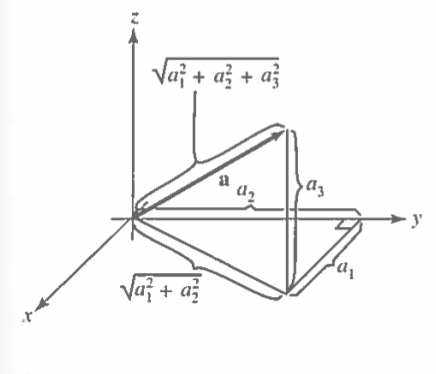
\includegraphics[width=1.1\textwidth]{fig_pyth.png}
\end{center}
\end{figure}
\end{columns}
\end{frame}

%------------------------------------------------
\begin{frame}
\frametitle{Orthogonal projection}
\begin{columns}[c]
\column{.45\textwidth} 
The orthogonal projection $\mathbf{p} $ of $\mathbf{w}$ on $\mathbf{v}$  is the vector whose tip is obtained by dropping a perpendicular line to the line $l$ (along v) from the top of $\mathbf{w}$. We can obtain the projection as:
$$  \mathbf{p} =\frac{ \mathbf{v} \cdot  \mathbf{w}}{\Vert \mathbf{v} \Vert^2}  \mathbf{v} $$

\column{.5\textwidth} 
\begin{figure}[htbp]
\begin{center}
 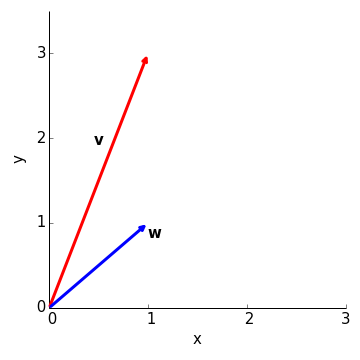
\includegraphics[width=\textwidth]{figure4a.png}
\caption{}
\end{center}
\end{figure}
\end{columns}
\end{frame}
%------------------------------------------------

%------------------------------------------------
\begin{frame}
\begin{columns}[c]
\column{.45\textwidth} 

So, 
	$\mathbf{v} = \left(
		\begin{array}{c}
		1\\
		3\\
		\end{array}
	\right)$

and 
	$\mathbf{w} = \left(
		\begin{array}{c}
		1\\
		1\\
		\end{array}
	\right)$\\
	

$$\mathbf{v} \cdot  \mathbf{w} = 1*1 + 3 *1 = 4 $$
$$\Vert \mathbf{v} \Vert^2 = 1^2 + 3^2 = 10 $$
$$  \mathbf{p} =\frac{\mathbf{v} \cdot  \mathbf{w}} {\Vert \mathbf{v} \Vert^2} \mathbf{v} =   \frac{4}{10} \left(
		\begin{array}{c}
		1\\
		3
		\end{array}
		\right)		
		= \left(
		\begin{array}{c}
		0.4\\
		1.2
		\end{array}
		\right)$$

\column{.45\textwidth} 
\begin{figure}[htbp]
\begin{center}
 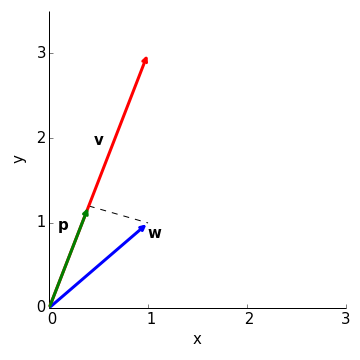
\includegraphics[width=\textwidth]{figure4b.png}
\caption{}
\end{center}
\end{figure}
\end{columns}
\end{frame}


%------------------------------------------------
\begin{frame}
\frametitle{Orthogonal vectors}
Two vectors $\mathbf{a}$ and $\mathbf{b}$ are orthogonal iff their inner product is equal to zero.
$$\mathbf{a} \cdot  \mathbf{b} = 0 $$
Then, the angle between $\mathbf{a}$ and $\mathbf{b}$ is equal to
$$ \cos\theta =\frac{\mathbf{a} \cdot \mathbf{b}}{\Vert \mathbf{a}\Vert  \Vert \mathbf{b} \Vert} = 0$$ from which we can see (remember trigonometry?!) that the angle is equal to 90$^{\circ}$. 

During this session we're going see how esp. the inner product is used in applications: {\color<1>[rgb]{1,0,0}{correlation, covariance, lineair (in)dependence, orthogonality}}  ,  {\color<1>[rgb]{0,0,1}{PCA and SVM}}.
\end{frame}

%------------------------------------------------
\section{Applications}
\begin{frame}
\frametitle{Correlation and the inner product}
Correlation is a measurement of linearity between random variables $x$ and $y$.
Traditionally, the correlation is defined as the covariance of the two variables dived by product of their standard deviations:
$$\rho(x,y) = \frac{cov(x,y)}{\sigma_x\sigma_y}$$
For limited (and zero-mean) samples, this unfolds as the correlation coefficient:
$$r(x,y) = \frac{ \frac{1}{n-1} \sum_i^n (x_i y_i)}
{\sqrt{\frac{1}{n-1}\sum_i^n x_i^2 } \sqrt{\frac{1}{n-1}\sum_i^n y_i^2}}$$
This looks familiar (apart from scaling $\frac{1}{n-1}$):
$$\mathbf{x} \cdot  \mathbf{y} = x_1 y_1 + x_2 y_2 + \ldots +  x_n y_n = \sum_i^n x_i y_i$$
\end{frame}

%------------------------------------------------
\begin{frame}
\frametitle{Correlation and the inner product}
So, it turns out that (for zero mean variables) the covariance is equal to the inner-product:
$$\mathbf{x} \cdot  \mathbf{y} = x_1 y_1 + x_2 y_2 + \ldots + x_n y_n= \sum_i^n x_i y_i = covar(x,y)$$

Something similar is happening to the standard deviations:
$$||x|| = \sqrt{x_^21 + x_2^2 \ldots} = \sqrt{\sum_i x_i^2}$$
So 
$$\sqrt{\sum_ix_i^2} \sqrt{\sum_iy_i^2} = ||x|| ||y||$$
\end{frame}


%------------------------------------------------
\begin{frame}
\frametitle{Correlation and the inner product}
by  combining the info so far we get:
$$r(x,y) = \frac{ \frac{1}{n-1}\sum_i x_i y_i}
{\sqrt{\frac{1}{n-1}\sum_i x_i^2} \sqrt{\sum_i y_i^2}} = \frac{\mathbf{x} \cdot  \mathbf{y} } {||x|| ||y||} = \cos{\theta}$$
The correlation coefficient can thus be calculated by taking the inner-product of two vectors and by dividing this by their norms. A graphical interpretation is the angle between them: the closer the two (n-dimensional) vectors, the more correlated they are.\\
Interactive example (iPython notebook)
\end{frame}

%------------------------------------------------
\begin{frame}
\begin{columns}[c]
\column{.4\textwidth} 
So far we've seen terms like orthogonality and correlation. They are related, but how?
\begin{block}{}
Linear independence
\end{block}

\begin{block}{}
Uncorrelated
\end{block}

\begin{block}{}
Orthogonal
\end{block}
\column{.55\textwidth} 
\begin{figure}[t]
\begin{center}
 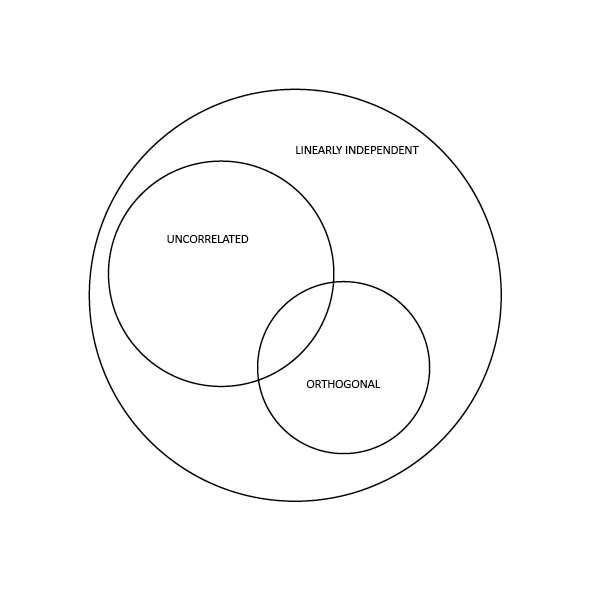
\includegraphics[width=1.3\textwidth]{relation_venn_stats_a}
\caption{}
\end{center}
\end{figure}
\end{columns}
\end{frame}


%------------------------------------------------
\begin{frame}
\begin{block}{Linear independence}
Two variables are linearly independent iff there is no constant $a$ such that
$$a \textbf{x} - \textbf{y} = 0$$
\end{block}

\begin{block}{Orthogonal}
Two variables are linearly orthogonal iff their inner product equals zero
$$\textbf{x} \cdot \textbf{y}= 0$$
\end{block}

\begin{block}{Uncorrelated}
Two variables are uncorrelated iff their demeaned inner product equals zero
$$(\textbf{x} - \overline{x} ) \cdot (\textbf{y} - \overline{y}) = 0$$
\end{block}
\end{frame}
%------------------------------------------------

\begin{frame}
\frametitle{Linear independence, orthogonality and correlation}
\begin{figure}[t]
\begin{center}
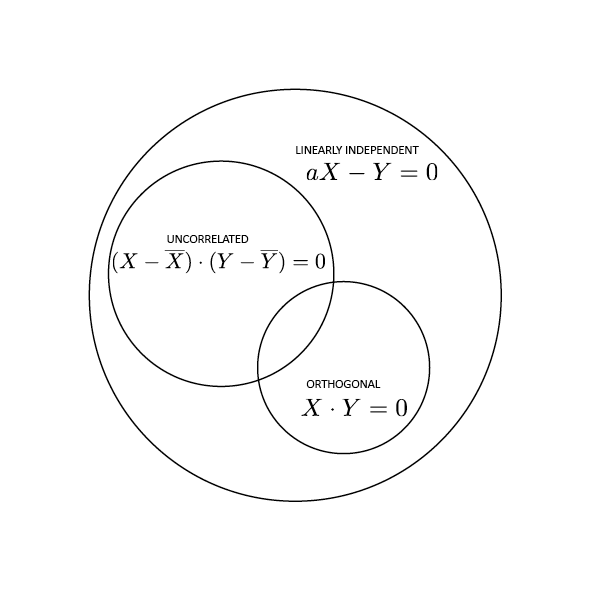
\includegraphics[width=0.7\textwidth]{relation_venn_stats_b}
\caption{}
\end{center}
\end{figure}

\end{frame}


%------------------------------------------------
\begin{frame}
\frametitle{Linear independence, orthogonality and correlation}
Thus, orthogonal denotes that the raw variables are perpendicular whereas uncorrelated denotes that the centred (=demeaned) variables are perpendicular! See e.g. Rodgers (1984) 
\url{https://www.psych.umn.edu/faculty/waller/classes/FA2010/Readings/rodgers.pdf}
examples:
\begin{itemize} 
\item $x = [1,1,2,3]$ and $y = [2,3,4,5]$?
\item $x = [0,0,1,1]$ and $y = [1,0,1,0]$?
\item $x = [1,-5,3, -1]$ and $y = [5,1,1,3]$?
\item $x = [-1,-1,1,1]$ and $y = [1,-1,1,-1]$?
\item $x = [1,2,3,4]$ and $y = [3,6,9,12]$?
\end{itemize}
\end{frame}

%------------------------------------------------
\begin{frame}
examples:
\begin{itemize} 
\item $x = [1,1,2,3]$ and $y = [2,3,4,5]$ :  independent, correlated and not orthogonal
\item $x = [0,0,1,1]$ and $y = [1,0,1,0]$ : independent, uncorrelated and not orthogonal
\item $x = [1,-5,3, -1]$ and $y = [5,1,1,3]$  : independent, correlated and orthogonal
\item $x = [-1,-1,1,1]$ and $y = [1,-1,1,-1]$ : independent, not correlated and orthogonal
\item $x = [1,2,3,4]$ and $y = [3,6,9,12]$ : not independent, correlated and not orthogonal
\end{itemize}
\end{frame}

%----------------------------------------------------------------------------------------
\begin{frame}
\frametitle{PCA, eigenvectors and eigenvalues}
PCA often boils down to rotation of data, such that the variance (std) is maximal along the first axis. 
Eigenvectors (principle components) are linear combinations of the original axes, such that variance is maximised and the corresponding eigenvalues are equal to the variances of the data along the eigenvectors. 
\begin{figure}[t]
\begin{center}
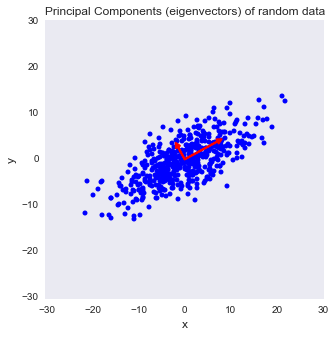
\includegraphics[width=0.5\textwidth]{pca}
\caption{}
\end{center}
\end{figure}
\end{frame}
%----------------------------------------------------------------------------------------

\begin{frame}
\frametitle{Support vector machines}
\begin{figure}[t]
\begin{center}
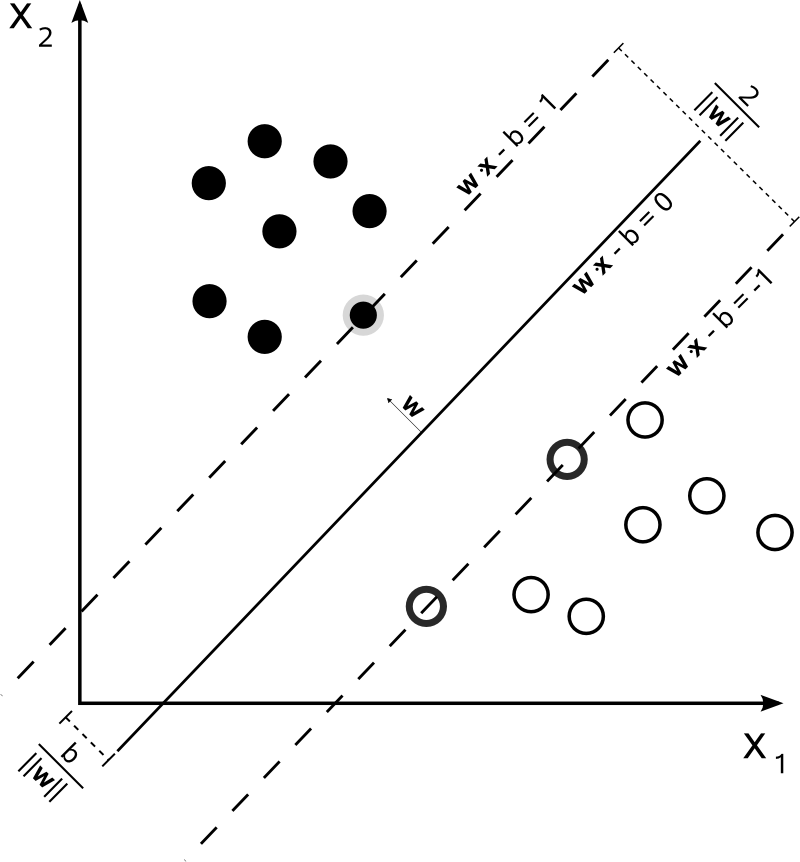
\includegraphics[width=0.65\textwidth]{svm}
\caption{}
\end{center}
\end{figure}
\end{frame}
%----------------------------------------------------------------------------------------
\begin{frame}
\frametitle{Geometry of the cross product}
The cross-product is defined as 
$$|| \mathbf{a} \times \mathbf{b}|| = || \mathbf{a} || ||\mathbf{b}|| \sin{\theta}$$    
\begin{figure}[htbp]
\begin{center}
 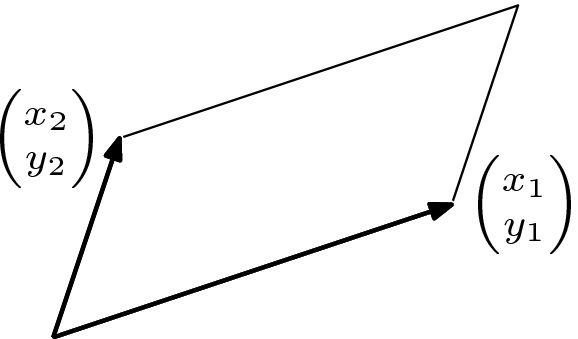
\includegraphics[width=0.7\textwidth]{parallelogram.png}
\caption{}
\end{center}
\end{figure}
\end{frame}

\begin{frame}
\frametitle{Geometry of the cross-product in 3D}
\begin{figure}[htbp]
\begin{center}
 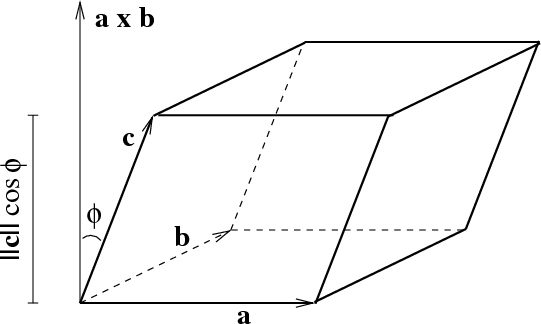
\includegraphics[width=\textwidth]{volume_parallelepiped.png}
\caption{}
\end{center}
\end{figure}

\end{frame}

\section{summary}
\begin{frame}
\frametitle{summary}
Today we've encountered vectors and various related properties:
\begin{itemize}
\item scalar multiplication
\item vector addition
\item inner product  $\mathbf{a} \cdot  \mathbf{b}$
\item outer product $\mathbf{a} \times \mathbf{b}$
\end{itemize}

\end{frame}

\begin{frame}
\frametitle{bonus infinite sum}
\begin{block}{Q}
What is the sum of all natural numbers $1+2+3 ... \inf$?
$$\sum_n^{\inf}n = - \frac{1}{12}$$
\end{block}
\end{frame}



\begin{frame}
\Huge{\centerline{Questions}}
\end{frame}
%------------------------------------------------


\end{document} 